\chapter{Evaluation}
The aim of evaluation was to compare the performance of my compiler with existing alternatives for running code on the web, and measure the impact of the optimisations implemented. Performance was based on three metrics: 

\begin{itemize}
\item \textbf{Execution time}: This was measured by a JavaScript program for each of the alternatives being considered, which were run using Node.js. Timing information is gotten from the \verb|performance| interface, which has up to microsecond precision and is not affected by system time changes so is guaranteed to be monotonic. This is sampled over 20 runs of the program and the mean and 95\% confidence interval are stored. \\
\item \textbf{Heap usage}: The amount of heap memory used was also collected by these scripts. Without garbage collection, my runtime allocates memory linearly so a call to allocate 0 bytes returns the total memory used. For the garbage collected allocator, I created a separate version which tracks the peak memory allocated, updating this on each memory allocation and accessible externally. 
The Grain runtime's development build outputs similar memory tracing statistics, from which the amount of heap memory used can be obtained. Even after removing some of the unnecessary tracing, its overhead is significant so this was done separately to collecting timing information. For C, where the standard library is included in the WebAssembly output for memory allocation, \verb|sbrk(0)| returns the size of the WebAssembly linear memory. Lastly, for programs converted to JavaScript, the test script is run with the \verb|--expose-gc| option. This allows calling the garbage collector before the program is executed, and approximating the memory used by calling \verb|process.memoryUsage().heapUsed| before and after the program runs. This is an approximate value, so it is also averaged over 20 iterations.
\item \textbf{Output file size}: This is easily obtained from the file system.

\end{itemize}


\section{Microbenchmarks}
I wrote a set of test programs, each aiming to represent a different programming style to see how performance varied across applications. The programs were parameterised so that comparisons could also be made at different problem sizes too. Only a few instances of this are included in the data to keep the number of dimensions of comparison manageable, instead focusing more on other aspects. The microbenchmarks used were:

% TODO: Rename everywhere so I can use other names instead
\begin{itemize}
\item \verb|alltrees|: Constructs a list of all binary trees of a given size, resulting in heavy memory usage and objects that exist for varying lifetimes.

\item \verb|arith|: Computes Euler's totient function for all integers from 1 to \verb|n|, involving a large amount of integer arithmetic. This was based on the solution to problem 34 of the 99 Problems in OCaml \nocite{99-problems}, which is to implement Euler's totient function.

\item \verb|composition|: Constructs a function which is the composition of a list of simple functions and maps it over a list, making heavy use of higher-order functions to define composition.

\item \verb|funcrec|: (functions, records) Compares three forms of parameterisation, using functions defined at the top-level of a program, using functions passed as arguments to another function, and using functions wrapped inside a record which is passed instead. This was based on an existing repository of OCaml benchmarks available on GitHub \nocite{chris00}.

\item \verb|mergesort|: Implements mergesort, making heavy use of lists and pattern matching.

\item \verb|nbody|: Solves the n-body, simulating the motion of planets for a number of time steps and making heavy use of floating point arithmetic. This was adapted from the benchmark program available in the Computer Language Benchmarks Game repository \nocite{benchmark-game}.
\end{itemize}

A couple other microbenchmarks were also used to demonstrate the worst-case behaviour some optimisations aim to avoid. These will be described later when the data for those optimisations is presented. 


\section{Comparison Against Alternatives}
Although most of the runtime for my compiler is written in WebAssembly, the garbage collected memory allocator is written in JavaScript due to its complexity and wanting to make several improvements to it. Therefore, the performance of my compiler is indicated with and without garbage collection, primarily to distinguish the overhead of calling between WebAssembly and JavaScript for each memory allocation. The data given is also for the optimised version of the compiler.

\subsection{Execution Time}

\begin{figure}[H]
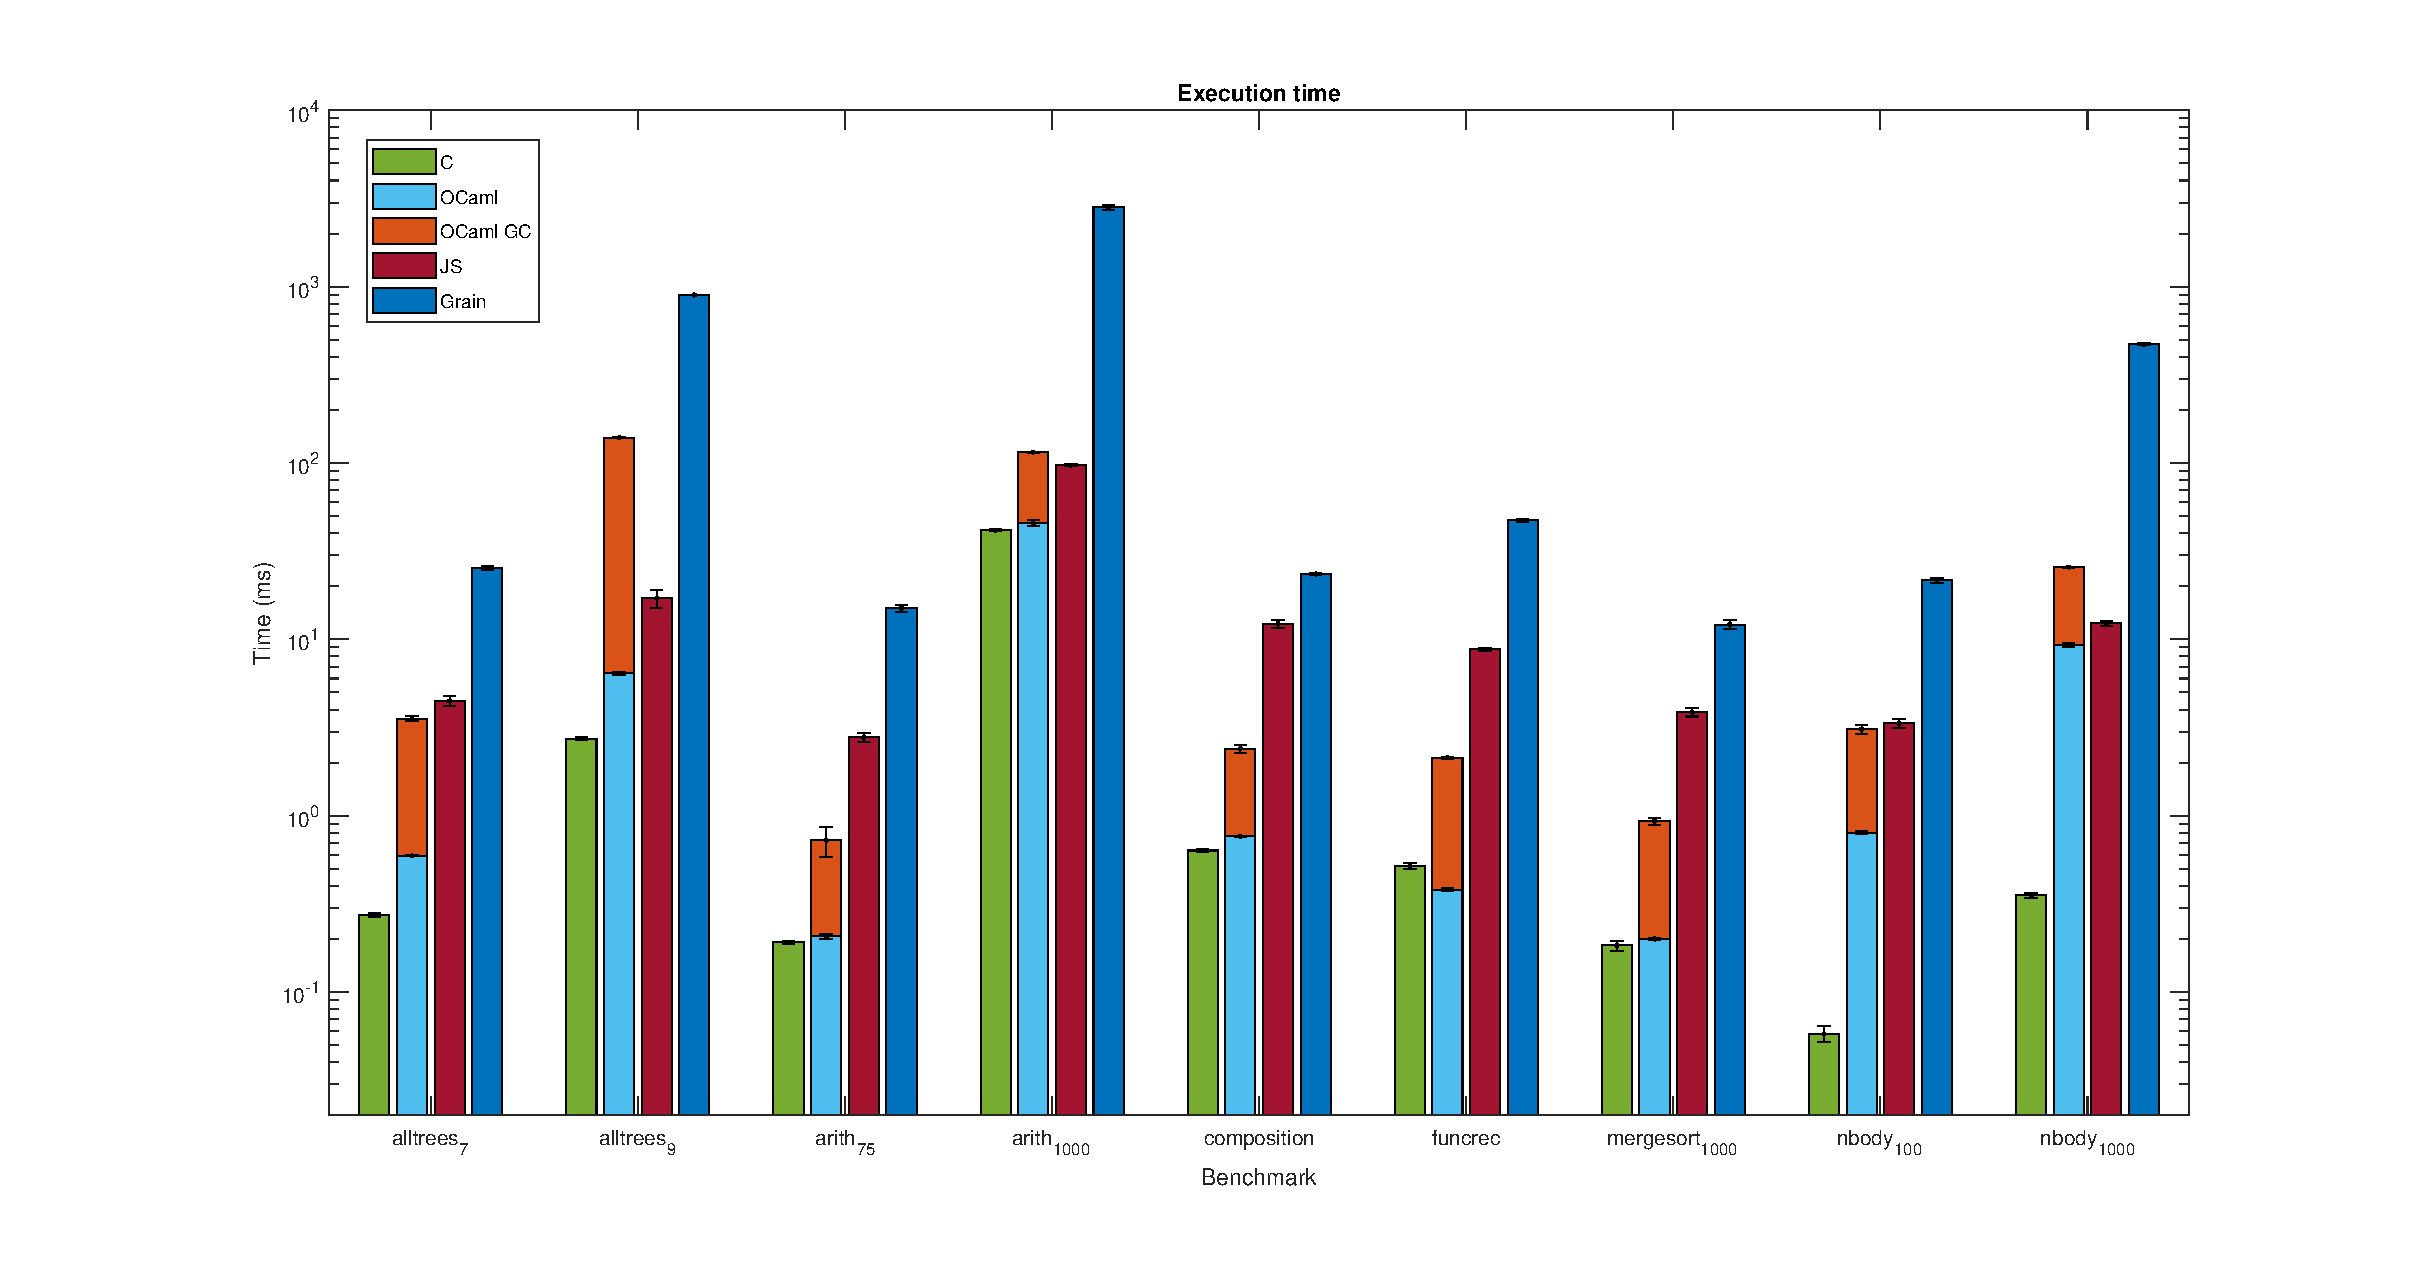
\includegraphics[scale=0.42]{figures/alternatives_timing}
\caption{Execution times for each alternative}
 \label{fig:alt_timing} 
\end{figure}

First, we see that the execution speed can vary by a couple orders of magnitude between the least and most efficient method. Unsurprisingly, the programs translated to C and compiled to WebAssembly through Clang/LLVM are the fastest. At the opposite extreme, Grain is always significantly slower than the other methods. Although my compiler is always faster than the equivalent JavaScript when run without garbage collection, the overhead of garbage collection results in the two being more balanced, performing better on some programs and worse on others. This is shown in more detail below:


\begin{figure}[H]
\hspace{-1.8cm}
\includegraphics[scale=0.52]{figures/js_ocaml_timing}
 \label{fig:js_oc_timing} 
\end{figure}

Without garbage collection, my compiler's output	executes between 0.33 and 20 times faster than the JavaScript program produced by translating the OCaml input program with Js\_of\_ocaml. With garbage collection, it still outperforms the JavaScript alternative in most cases, except for programs making a very large number of memory allocations such as \verb|alltrees| with a large problem size.


\subsection{Heap Usage}

\begin{figure}[H]
\hspace{-1cm}
\includegraphics[scale=0.48]{figures/alternatives_heap}
 \label{fig:alt_heap} 
\end{figure}

There are no bars for C for \verb|arith| and \verb|funcrec|, as these did not require the heap to implement. 
% TODO: Should try to get some value for Grain Arith_1000, even if very few iterations
There is also no data for Grain for \verb|arith_1000| as the program was very slow without tracing (see \ref{fig:alt_timing}) and did not appear to terminate when run with tracing enabled.

With the exception of those C programs not requiring the heap, the garbage collected runtime uses at worst 13\% more memory than the C implementation, and uses significantly less memory than both the JavaScript and Grain alternatives. In every test (ignoring the Grain result for \verb|arith_1000|), the garbage collected runtime uses at most one third of the memory used by either the JavaScript or Grain version. 

The order of the bars for my compiler with and without garbage collection are reversed in four of the tests. These tests have fewer opportunities for garbage collection so the garbage collected runtime saves little memory, but consumes more due to the overhead of headers and trailers on allocated blocks. In the worst case, \verb|funcrec| has no opportunities for garbage collection and only allocates small objects of at most 8 bytes. Since each header and trailer is 8 bytes, garbage collection triples the amount of memory used.



\subsection{Output File Size}

\begin{figure}[H]
\hspace{-1cm}
\includegraphics[scale=0.48]{figures/alternatives_size}
 \label{fig:alt_size} 
\end{figure}

As expected, the JavaScript output is generally the largest as JavaScript is a text format rather than a binary format like WebAssembly. On average, it is 8 times larger than the output of my compiler with garbage collection enabled. Grain also produces much larger binary files, averaging about 3.5 times larger than my compiler's output. Inspecting the compiled output, there appears to be a few reasons for this. First, programs import a larger set of functions from Grain's runtime than used in my compiler as it supports more types of numerical data, such as having both 32-bit and 64-bit integers. It also uses a reference counting garbage collector, which adds more overhead since updating a value requires both incrementing the new value and decrementing the old value, whereas my garbage collector just overwrites the old value on the shadow stack. Lastly, it does not appear to optimise the WebAssembly produced, compared with my compiler which uses a register allocation algorithm to reduce the number of local variables declared, and peephole optimises trivially useless statements such as \verb|local.get i; drop|.

Compared with the output of compiling a C program, the sizes are similar except where the \verb|stdlib| library had to be included for memory allocation, which makes those programs about 7KB larger. For comparison, my runtime without garbage collection is a 740B WebAssembly file, but the garbage collector is implemented in JavaScript which when minified adds a 4KB file.

Lastly, this demonstrates the overhead of garbage collection in terms of the extra bookkeeping operations added to maintain the shadow stack. On average, this adds about 30\% to the size of the output WebAssembly.

\section{Optimisations}

I first compare the impact of the IR and WebAssembly optimisations separately, as well as their combined impact on performance. After that, I look at the impact of specific optimisations at the IR level by seeing how performance changes when one is removed. Finally, I show the benefit of going through all of the optimisations multiple times. %, as well as looking at how the phase ordering at the IR level impacts performance.  -- LEAVE THIS FOR IF SECTION TOO SHORT
Data is collected with garbage collection disabled to exclude the overhead it introduces.

\subsection{IR and WebAssembly optimisations}

\begin{figure}[H]
\hspace{-1cm}
\includegraphics[scale=0.5]{figures/opts_threeplots}
 \label{fig:opts} 
\end{figure}

The peephole optimisations done at the WebAssembly level have very little impact on memory usage or execution time, but consistently reduce output size by about 10\%. The IR optimisations improve execution time and heap usage by at least 30\% for five of the microbenchmarks, but fail to improve \verb|mergesort| or \verb|nbody|. In a couple of cases, inlining or rewriting functions completely removes the need to construct closures recursively, resulting in near zero heap usage for those programs. The execution time of \verb|nbody| is the one case where the optimisations decrease performance, but only by 3\%.  \verb|nbody| is an imperative style program, which may explain why the optimisations perform well on the other programs but not on it, since they avoid trying to optimise the use of mutable values and the program has no recursion to optimise.

\subsection{Impact of inlining, uncurrying and tail calls}

\begin{figure}[H]
\hspace{-1cm}
\includegraphics[scale=0.62]{figures/specific_opts}
 \label{fig:specific-opts} 
\end{figure}

% NEED TO DESCRIBE INLINING AND JUSTIFY HEURISTICS! DON'T SEEM TO BE DOING MUCH HERE
This shows the change when one optimisation is removed, so the magnitude of each bar can be viewed as the speed-up or size reduction that optimisation adds on top of the other optimisations present. First, we see that where inlining increases file size (\verb|funcrec| and \verb|mergesort|), it is only by 5\% so the optimisation is not resulting in significant code bloat. Instead, inlining sometimes reduces the size of the output in cases where it completely removes a function definition. Overall it has a relatively small impact on performance, with the biggest change being a 15\% speed-up for \verb|funcrec|, suggesting that either the heuristics for inlining were too restrictive or that this set of microbenchmarks or other optimisations are not complex enough to see significant improvements from inlining.

% Getting too specific? Talk in higher-level general details?
Tail call optimisation does not affect several of the programs, but does improve the execution speed of \verb|funcrec| and the speed and file size for \verb|arith|. A more important factor, not demonstrated by the data shown, is that tail call optimisation allows some programs to execute that would otherwise give an error. \\
\verb|let rec f x = if x = 0 then 0 else f (x-1)| \\
Without tail call optimisation, calling this function with a large enough input causes the stack space to be used up and the program fails. With tail call optimisation, the function uses a fixed amount of space so can handle any input size.

Lastly, uncurrying fully applied functions has the most significant impact on performance. None of the programs are negatively impacted by it, yet it provides up to a 50\% improvement in execution speed for some tests. Additionally, not having to construct a closure for each separate argument reduces the amount of space used on the heap. In the case of \verb|arith|, this removes the need to recursively construct closures, resulting in an improvement which grows with the problem size. Once again, \verb|mergesort| and \verb|nbody| are not improved as they lack opportunities for this optimisation to be applied.


\subsection{Impact of number of passes}
Only one instance of each benchmark is shown, as the pattern is identical for other problem sizes.

\begin{figure}[H]
\hspace{-1cm}
\includegraphics[scale=0.65]{figures/iterations}
 \label{fig:iterations} 
\end{figure}

In almost all cases, there is no further improvement after iterating over the optimisations 3 times, with the exception of the file size for \verb|funcrec|. Therefore, 3 was chosen as the number of times to loop over the optimisation passes. By performing each optimisation three times, every optimisation happens both before and after every other one, so the effect of phase ordering is also reduced. This is important since there are several different passes being performed at the IR level, and many more benchmark programs would likely be needed to distinguish the best permutation of them.\\
Having multiple iterations also picks up cases where a value is propagated through several variables before being used e.g. \verb|let y = x in let z = y in f(z)|. The first pass would replace \verb|f(z)| with \verb|f(y)| but another pass is needed to replace this with \verb|f(x)| and remove both \verb|y| and \verb|z|.

% TODO: Phase ordering or not?

\section{Garbage Collection}










